\section{Surface} \label{sec:Surface}

Surface utility determines the average surface of structures such as
membranes or polymer brushes and calculates the surface areas.

The utility cuts the plane perpendicular to the chosen axis into squares of
size \tt{<width>*<width>} and then finds the beads with the highest and
lowest coordinates along the chosen axis whose other two coordinates fall
into the square for each square on the plane. By default, it searches the
chosen axis for the beads with the highest coordinate in the interval
$\langle0, (box length)/2\rangle$ and with the lowest coordinate in the
interval $\langle(box\ length)/2; (box\ length)\rangle$, i.e., it assumes
something such as a polymer brush on each wall. If \tt{--in}
option is used, it searches for a layer structure inside the box, i.e., it
searches for the bead with the lowest and highest coordinates in the whole
box, $\langle0; (box\ length)\rangle$ (this mode finds surfaces for
something like a bilayer).

Note that the utility does not determine any structures for now, therefore
any molecules outside the brush/membrane can be recognized as a part of the
surface (\tt{-bt} and \tt{-m} can be sometimes used to eliminate
this problem).

By default, all bead types and all molecule types are used, but using
\tt{-bt} and \tt{-m} options, only specified bead and/or molecule
types can be used. This is particularly useful when, e.g., other molecules
solubilize inside the brush/membrane, leaving some molecules in the
solution.

Following are two examples of usage with and without \tt{--in} option
(on top are snapshots with coloured balls representing the detected surface
and on the bottom are graphs of the surface):

\begin{minipage}{0.45\textwidth}
  \centering
  \tt{Surface in.vcf 1 out.txt z --in}
  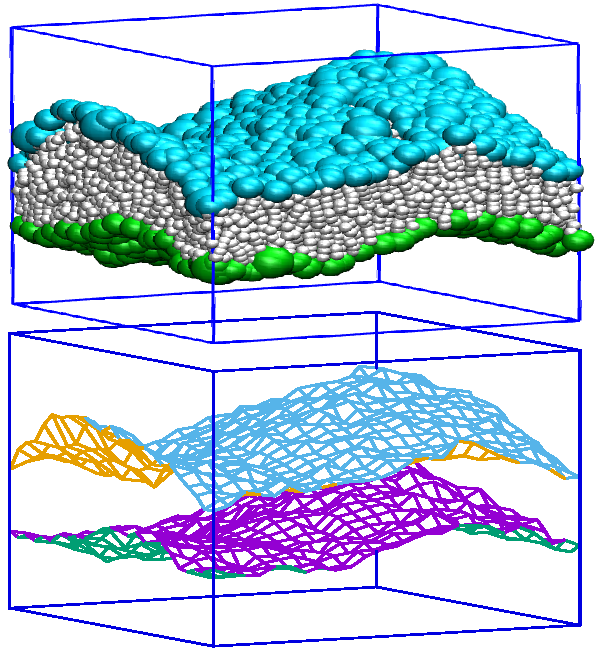
\includegraphics[width=\textwidth]{Surface-bilayer.pdf}
\end{minipage}
\hfill
\begin{minipage}{0.45\textwidth}
  \tt{Surface in.vcf 1 out.txt z}
  \centering
  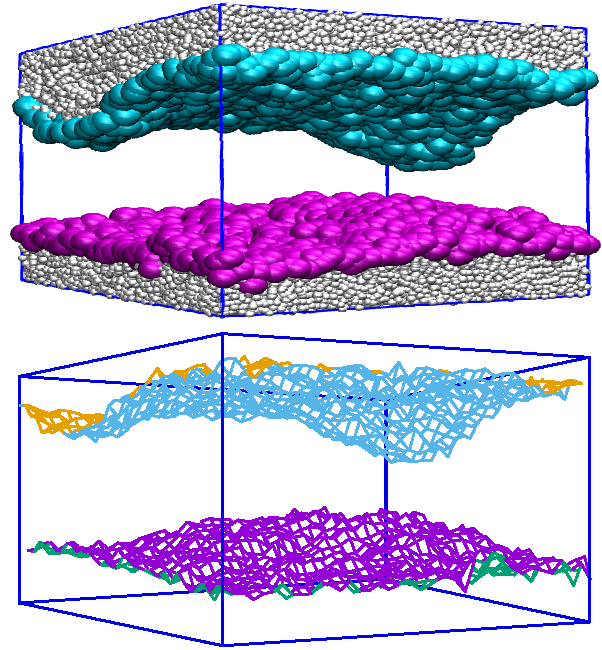
\includegraphics[width=\textwidth]{Surface-brush.pdf}
\end{minipage}

Usage:

\vspace{1em}
\noindent
Usage: \tt{Surface <input> <width> <surf.txt> <area.txt> <axis> [options]}
\noindent
\begin{longtable}{p{0.2\textwidth}p{0.744\textwidth}}
  \toprule
  \multicolumn{2}{l}{Mandatory arguments} \\
  \midrule
  \tt{<input>}    & input coordinate file (either \tt{vcf} or \tt{vtf} format)\\
  \tt{<width>}    & side length of each square\\
  \tt{<surf.txt>} & output file with average surface\\
  \tt{<area.txt>} & output file with per-timestep areas\\
  \tt{<axis>}     & direction in which to determine the surface: \tt{x}, \tt{y},
    or \tt{z}\\
  \toprule
  \multicolumn{2}{l}{Options} \\
  \midrule
  \tt{--in}          & start from the box centre instead of from its edges \\
  \tt{--bonded}      & use beads in molecules for surface recognition \\
  \tt{-bt <name(s)>} & use specified bead types for surface recognition \\
  \midrule
  \multicolumn{2}{l}{Other options (see the beginning of
                     Chapter~\ref{chap:Utils})}\\
  \midrule
  \multicolumn{2}{p{0.948\textwidth}}{\tt{-st},
                                      \tt{-e},
                                      \tt{-sk},
                                      \tt{-i},
                                      \tt{--verbose},
                                      \tt{--silent},
                                      \tt{--help},
                                      \tt{--version}}\\
  \bottomrule
\end{longtable}

\noindent
Format of output files:
\begin{enumerate}[nosep,leftmargin=20pt]
  \item \tt{<surf.txt>} -- 3D coordinates
    \begin{itemize}[nosep,leftmargin=5pt]
      \item first line: AnalysisTools version
      \item second line: command used to generate the file
      \item third line: column headers
        \begin{itemize}[nosep,leftmargin=5pt]
          \item first two numbers represent the centre of each square
            (being the coordinates on the sliced up plane); i.e., if
            \tt{<width>} is 1, then the centre of the first square is 0.5 0.5,
            the centre of
            the second one is 0.5 1.5, etc.
          \item the second two numbers are coordinates of the surface in
            the third dimension, i.e., along the chosen axis
        \end{itemize}
        \item data lines follow
    \end{itemize}
  \item \tt{<area.txt>} -- per-timestep areas (calculated as a sum of triangles)
    \begin{itemize}[nosep,leftmargin=5pt]
      \item first line: AnalysisTools version
      \item second line: command used to generate the file
      \item third line: column headers
        \begin{itemize}[nosep,leftmargin=5pt]
          \item first is simulation timestep
          \item the rest are areas of the top, bottom, and central surfaces
        \end{itemize}
        \item data lines follow
        \item second to last line: column headers for overall averages
        \item last line: the overall averages
    \end{itemize}
\end{enumerate}
